\documentclass{../source/zjureport}

\major{信息工程}
\name{周灿松}
\title{实验设计报告}
\stuid{3190105055}
\college{信息与电子工程学院}
\date{\today}
\lab{教4-421}
\course{数字信号处理}
\instructor{徐元欣}
\grades{}
\expname{有限长序列、频谱、DFT的性质}
\exptype{演示}
\partner{--}

\begin{document}
    \makeheader
    \section{实验目的和要求}
    设计通过演示实验,建立对典型信号及其频谱的直观认识,理解DFT的物理意义、主要性质。

    \section{实验内容和步骤}
        \begin{figure}[!htp]
            \centering
            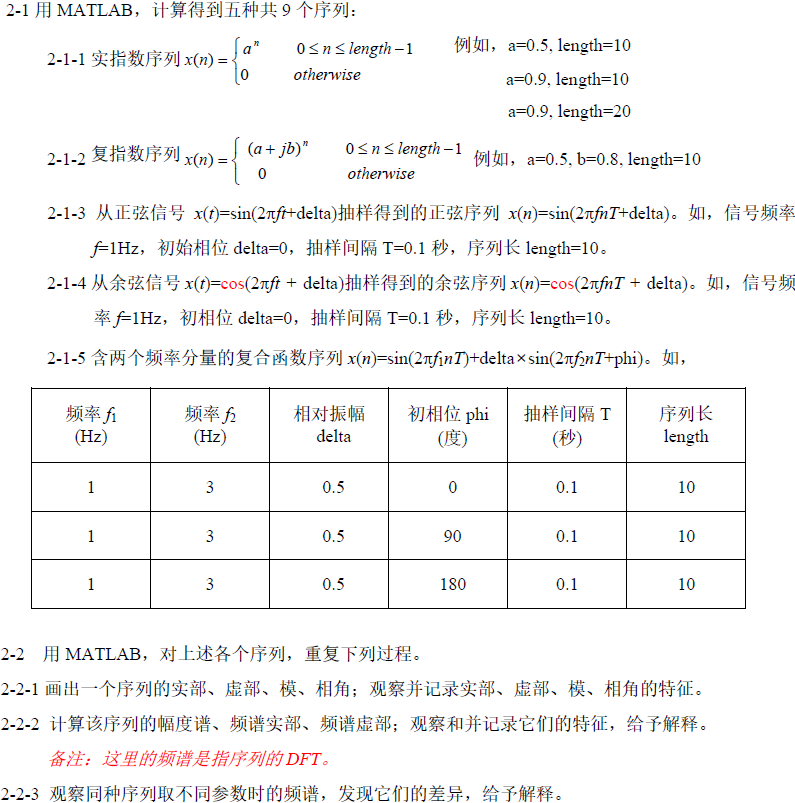
\includegraphics[width = 0.8\textwidth]{figure/page1.png}
        \end{figure}
        \newpage
    
    \section{主要仪器设备}
    MATLAB编程。
    \section{操作方法和实验步骤}
    (参见“二、实验内容和步骤”)
    \section{实验数据记录和处理}
        \lstinputlisting[caption = 主体代码,language=matlab]{code/Problem1.m}
        \newpage
        \lstinputlisting[caption = 产生实指数序列的函数,language = matlab]{code/realExpSeq.m}
        \lstinputlisting[caption = 产生复指数序列的函数,language=matlab]{code/comExpSeq.m}
        \lstinputlisting[caption = 产生正弦序列的函数,language=matlab]{code/sinSeq.m}
        \lstinputlisting[caption = 产生余弦序列的函数,language=matlab]{code/cosSeq.m}
        \lstinputlisting[caption = 产生复合函数序列的函数,language=matlab]{code/comFunc.m}
        \lstinputlisting[caption = 绘制序列的实部、虚部、模、相角的函数,language=matlab]{code/plotPart.m}
        \lstinputlisting[caption = 绘制序列的幅度谱、频谱实部、频谱虚部的函数,language=matlab]{code/dftPlot.m}
    \section{实验结果与分析}
        \subsection{各个序列图形及解释}
            \subsubsection{实指数序列}
                \begin{figure}[htbp]
                    \centering
                    \begin{minipage}[t]{0.48\textwidth}
                    \centering
                    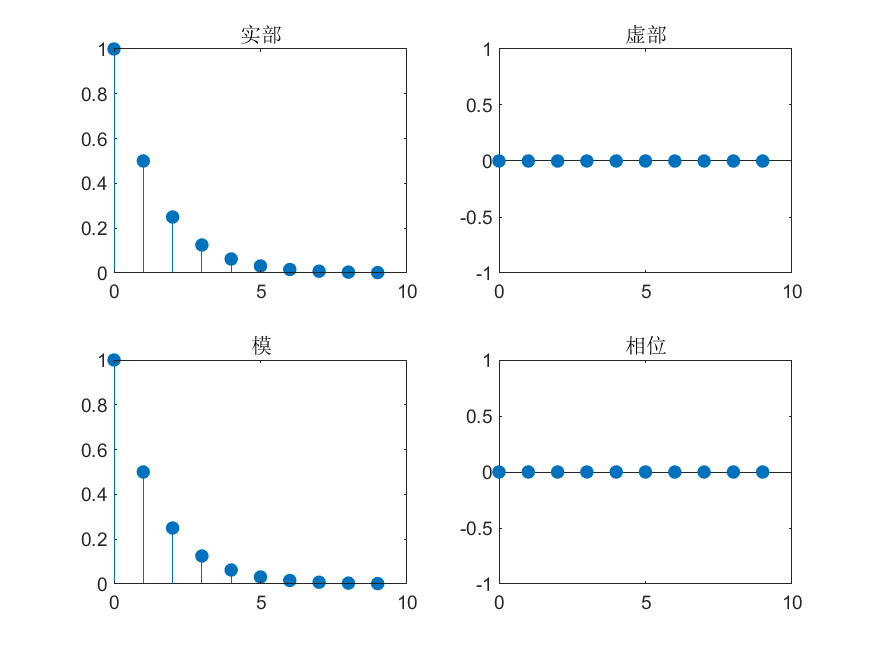
\includegraphics[width=\textwidth]{figure/实指数序列_a=05,length=10.png}
                    \end{minipage}
                    \begin{minipage}[t]{0.48\textwidth}
                    \centering
                    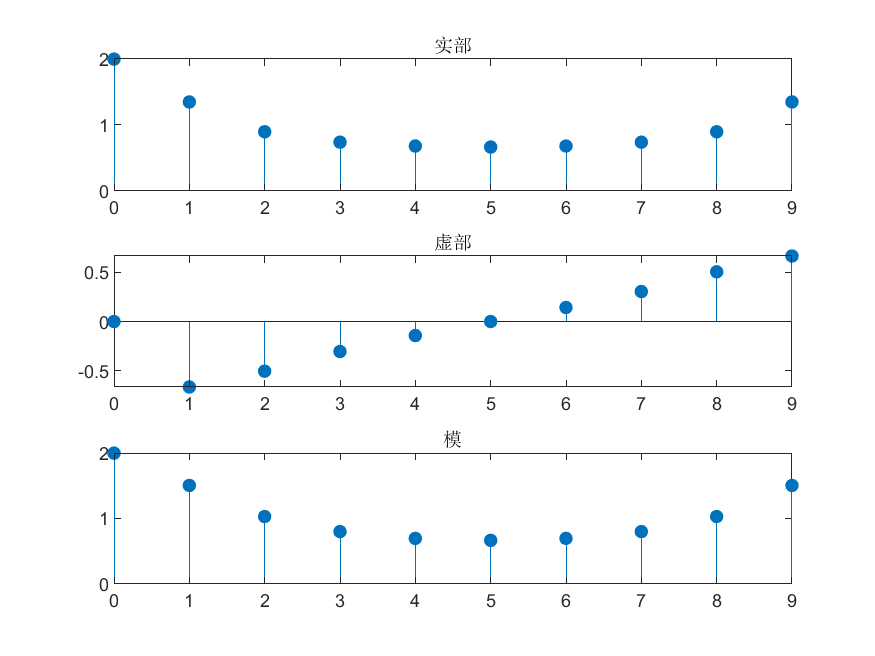
\includegraphics[width=\textwidth]{figure/频谱_实指数序列_a=05,length=10.png}
                    \end{minipage}
                    \caption{a=0.5,length=10}
                \end{figure}

                \begin{figure}[htbp]
                    \centering
                    \begin{minipage}[t]{0.48\textwidth}
                    \centering
                    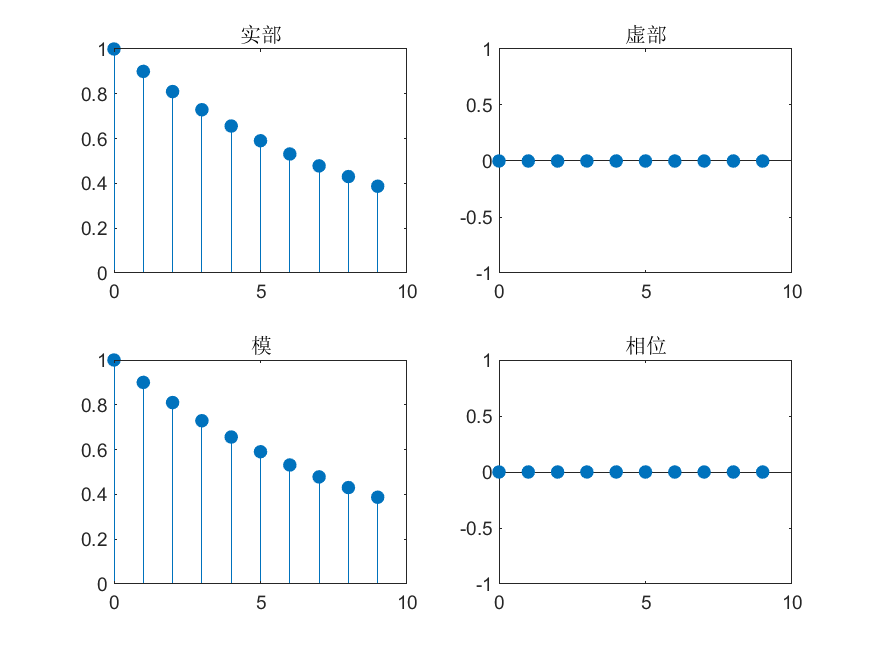
\includegraphics[width=\textwidth]{figure/实指数序列_a=09,length=10.png}
                    \end{minipage}
                    \begin{minipage}[t]{0.48\textwidth}
                    \centering
                    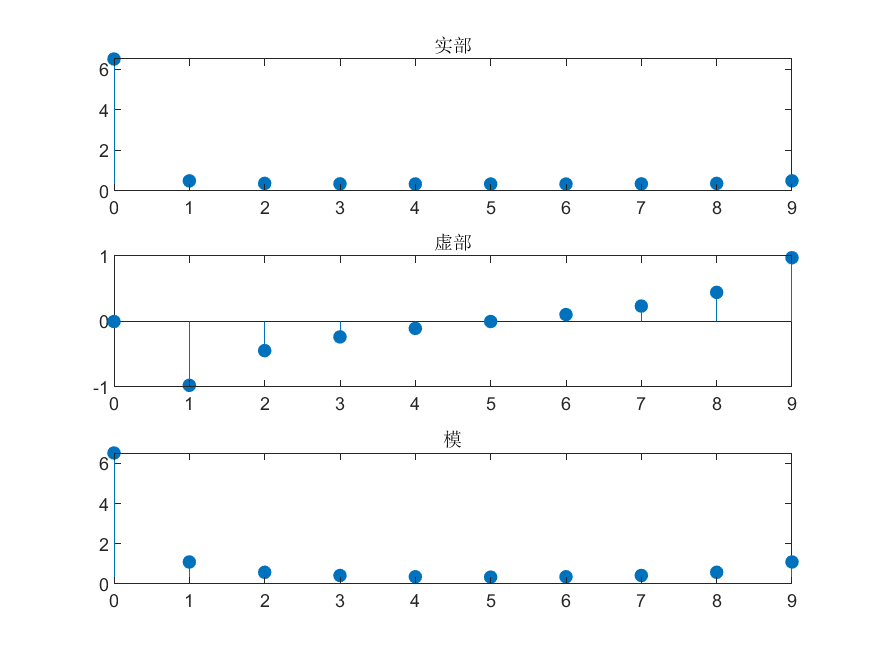
\includegraphics[width=\textwidth]{figure/频谱_实指数序列_a=09,length=10.png}
                    \end{minipage}
                    \caption{a=0.9,length=10}
                \end{figure}
                
                \newpage

                \begin{figure}[htbp]
                    \centering
                    \begin{minipage}[t]{0.48\textwidth}
                    \centering
                    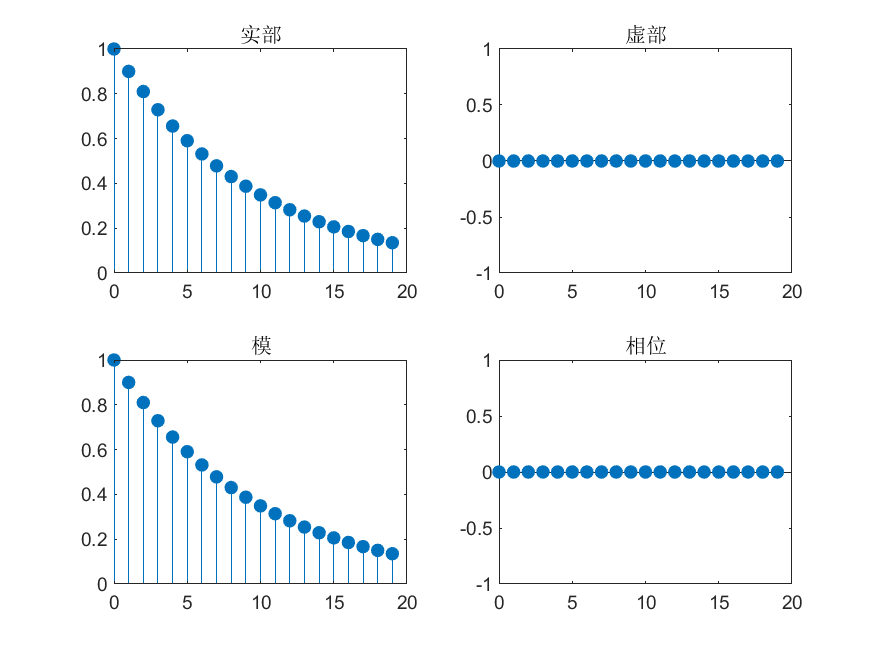
\includegraphics[width=\textwidth]{figure/实指数序列_a=09,length=20.png}
                    \end{minipage}
                    \begin{minipage}[t]{0.48\textwidth}
                    \centering
                    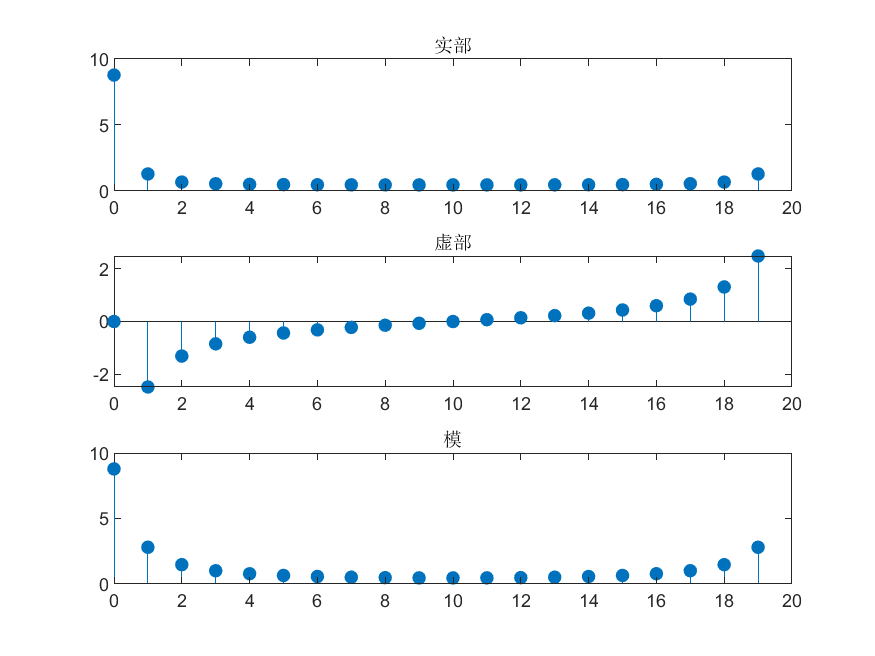
\includegraphics[width=\textwidth]{figure/频谱_实指数序列_a=09,length=20.png}
                    \end{minipage}
                    \caption{a=0.9,length=20}
                \end{figure}

                【\textbf{分析}】
                
                观察三个序列的时域图像,因为这三个序列均为实指数序列,所以它们的虚部和相位均为0;a的值越大,实部(模)的相位衰减就越慢,就越接近直流分量。

                观察三个序列的频域图像,可以发现他们的实部偶对称,虚部奇对称。结合所学的知识,我们可以得出知道这是由于该序列在是实数序列的原因。同时,我们可以发现当a的值增大时,X(0)的值也越大,也就是说序列的直流分量更大。除此之外,我们也可以发现length越大,频谱就越接近真实图像,这是由于采样率的提升。
            
            \subsubsection{复指数序列}
                \begin{figure}[htbp]
                    \centering
                    \begin{minipage}[t]{0.48\textwidth}
                    \centering
                    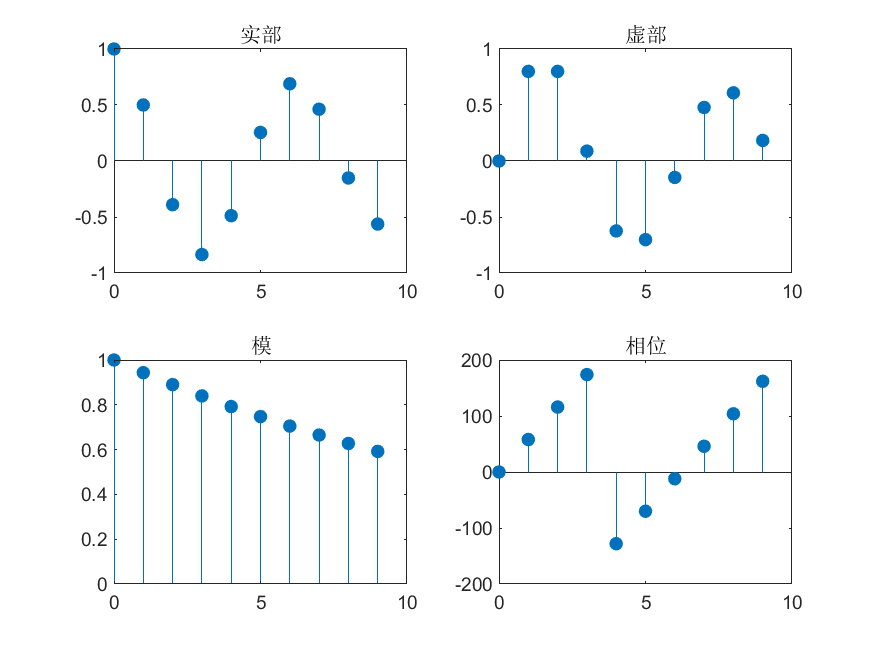
\includegraphics[width=\textwidth]{figure/复指数序列.png}
                    \end{minipage}
                    \begin{minipage}[t]{0.48\textwidth}
                    \centering
                    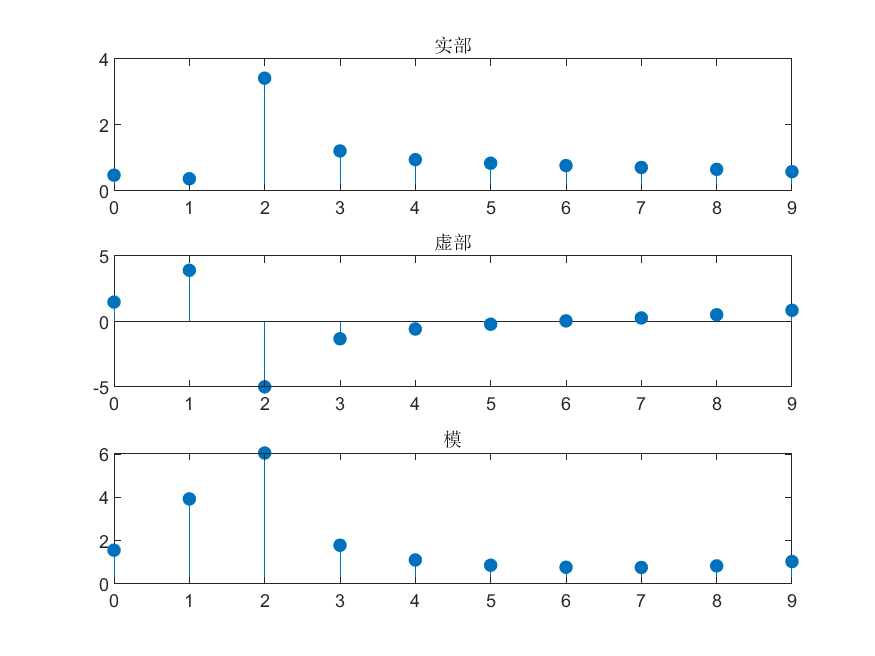
\includegraphics[width=\textwidth]{figure/频谱_复指数序列.png}
                    \end{minipage}
                    \caption{复指数序列}
                \end{figure}


                【\textbf{分析}】
                该序列为复指数序列,其可表示为$\sqrt{a^2+b^2}e^{jn\theta} =\sqrt{a^2+b^2}(cos(n\theta)+j\sin(n\theta))$的形式,所以时域的实部与虚部表现为正弦函数的抽样结果,相位呈现线性,因为$\sqrt{a^2+b^2}<1$,所以模减小。频域上未发现明显特点。
                

            \subsubsection{正弦序列图像}
                \begin{figure}[htbp]
                    \centering
                    \begin{minipage}[t]{0.48\textwidth}
                    \centering
                    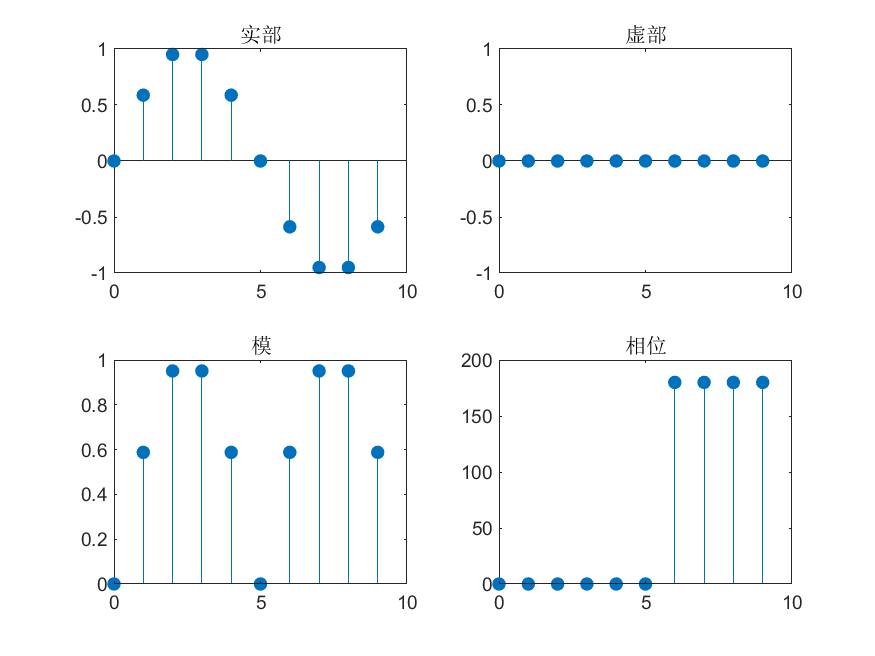
\includegraphics[width=\textwidth]{figure/正弦序列.png}
                    \end{minipage}
                    \begin{minipage}[t]{0.48\textwidth}
                    \centering
                    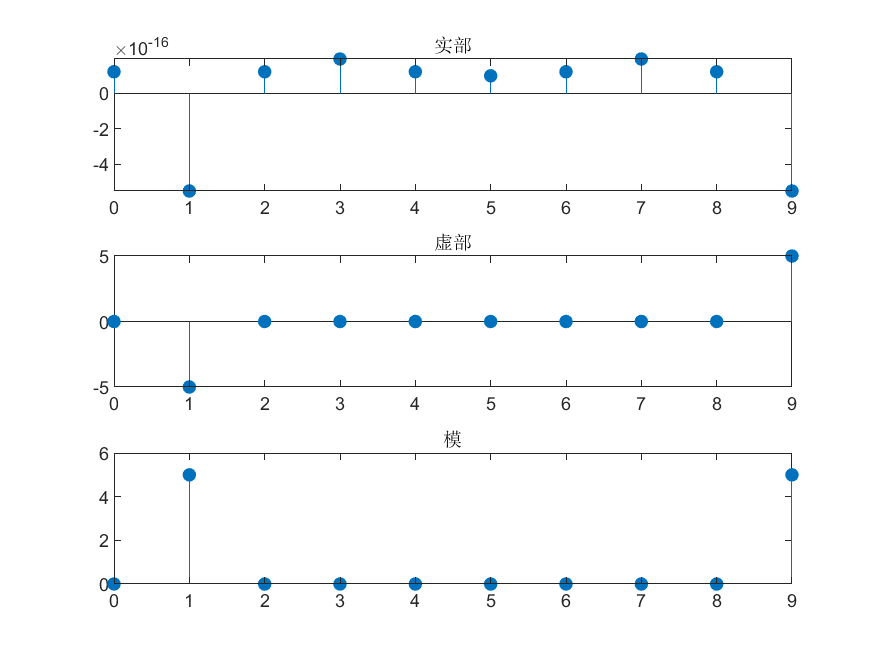
\includegraphics[width=\textwidth]{figure/频谱_正弦序列.png}
                    \end{minipage}
                    \caption{正弦序列}
                \end{figure}
                【\textbf{分析}】

                该序列是正弦函数的采样,采样周期为0.1s。观察时域图像可知:该序列为奇对称的实序列,在x(n)大于零时相位为0,小于零时相位为180°。

                因为该序列的对称性,所以频谱的实部应该为0,且虚部奇对称。虚部值出现在1Hz处,与原序列频率吻合。
                

            \subsubsection{余弦序列}
                \begin{figure}[htbp]
                    \centering
                    \begin{minipage}[t]{0.48\textwidth}
                    \centering
                    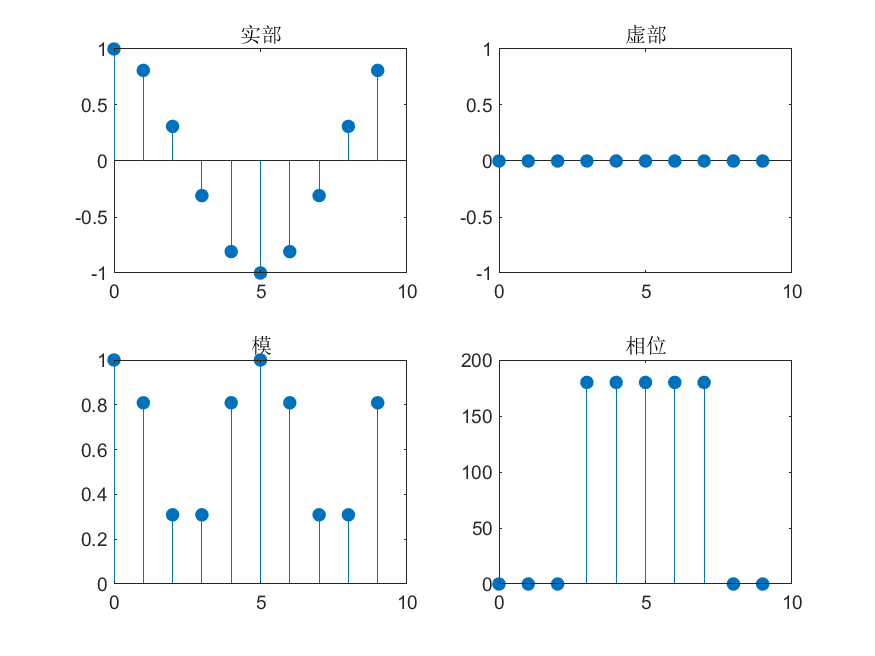
\includegraphics[width=\textwidth]{figure/余弦序列.png}
                    \end{minipage}
                    \begin{minipage}[t]{0.48\textwidth}
                    \centering
                    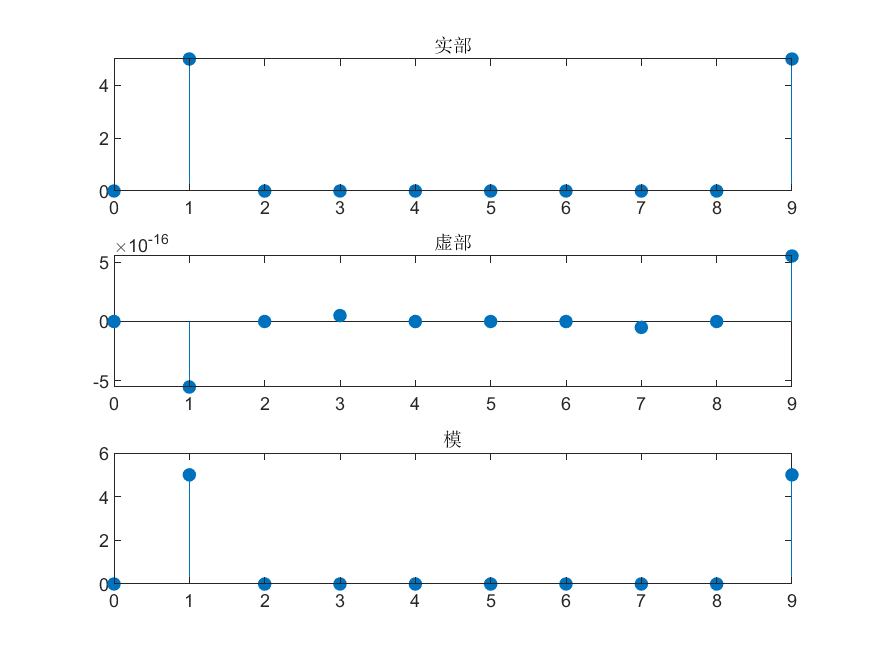
\includegraphics[width=\textwidth]{figure/频谱_余弦序列.png}
                    \end{minipage}
                    \caption{余弦序列}
                \end{figure}

                【\textbf{分析}】
                观察时域,可得该序列是偶对称的实序列,虚部为0,相位与正弦函数类似。因为它的对称性,频域的虚部理论上应该为0,此处不为零是由于MATLAB是数值计算,有一定的误差,可以看出虚部的值是一个极小的值。谱线出现在1Hz处,与原序列的频率吻合。



            \subsubsection{复合函数序列}
                \begin{figure}[htbp]
                    \centering
                    \begin{minipage}[t]{0.48\textwidth}
                    \centering
                    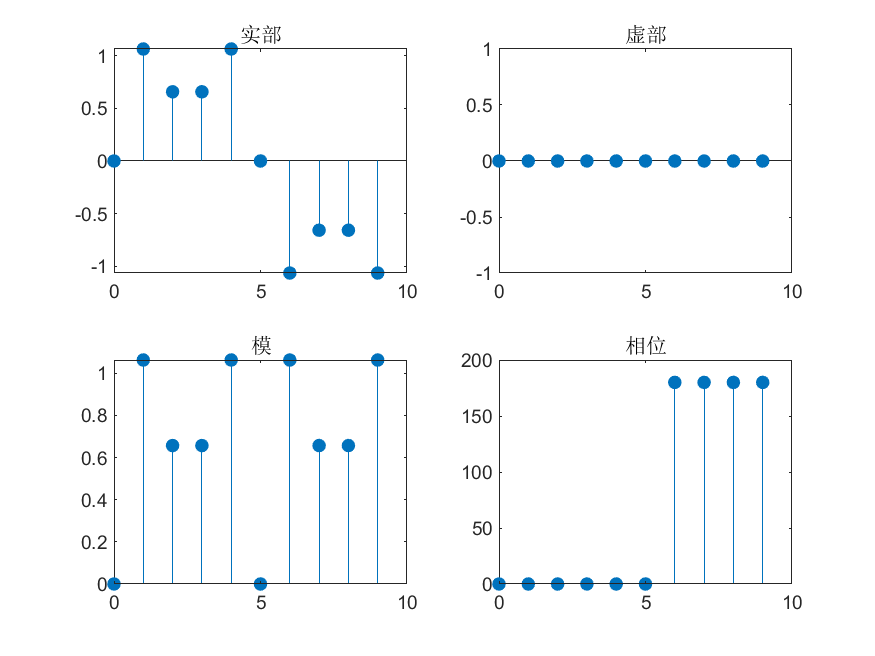
\includegraphics[width=\textwidth]{figure/复合函数序列_phi=0.png}
                    \end{minipage}
                    \begin{minipage}[t]{0.48\textwidth}
                    \centering
                    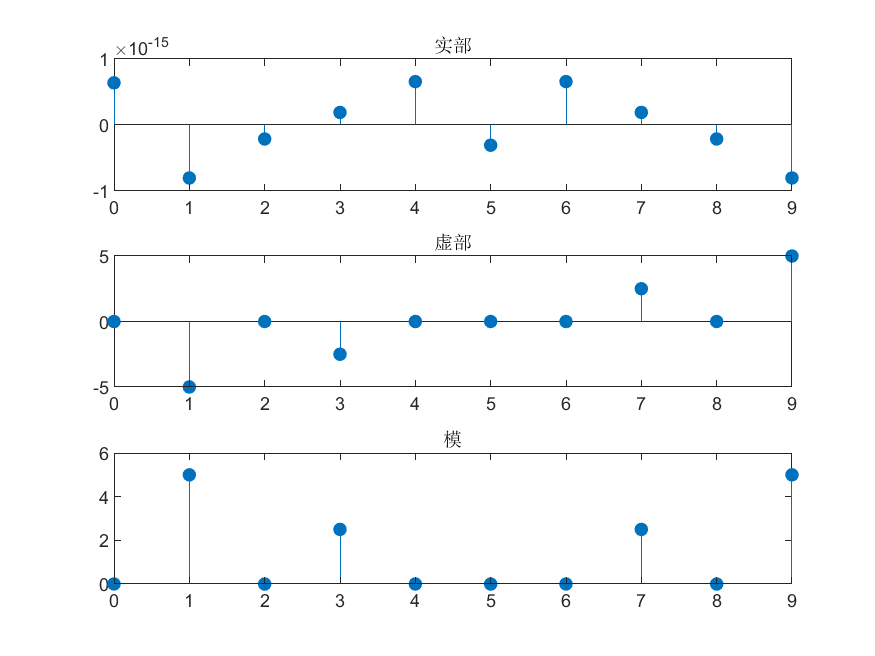
\includegraphics[width=\textwidth]{figure/频谱_复合函数序列_phi=0.png}
                    \end{minipage}
                    \caption{phi=0}
                \end{figure}

                \newpage

                \begin{figure}[htbp]
                    \centering
                    \begin{minipage}[t]{0.48\textwidth}
                    \centering
                    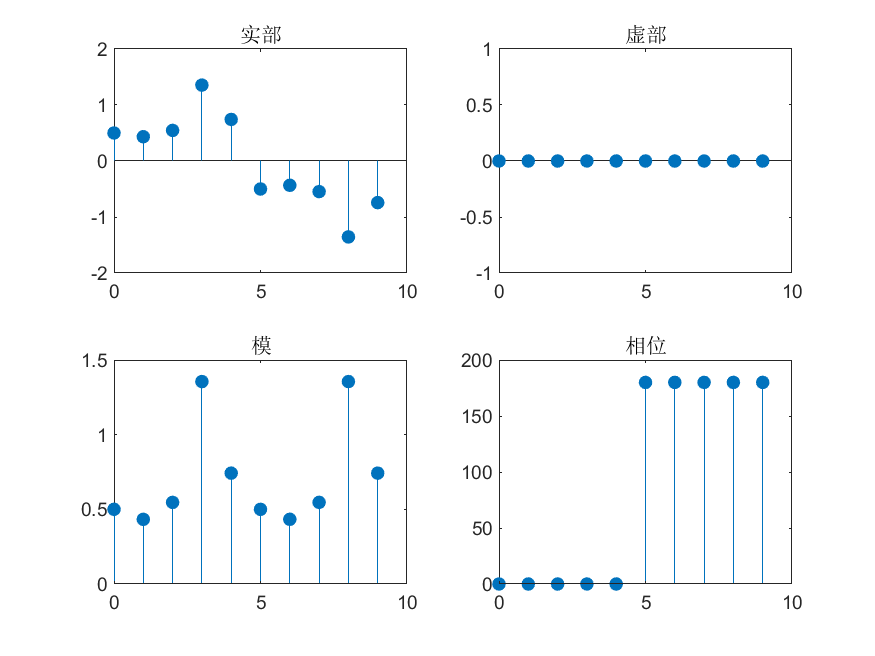
\includegraphics[width=\textwidth]{figure/复合函数序列_phi=90.png}
                    \end{minipage}
                    \begin{minipage}[t]{0.48\textwidth}
                    \centering
                    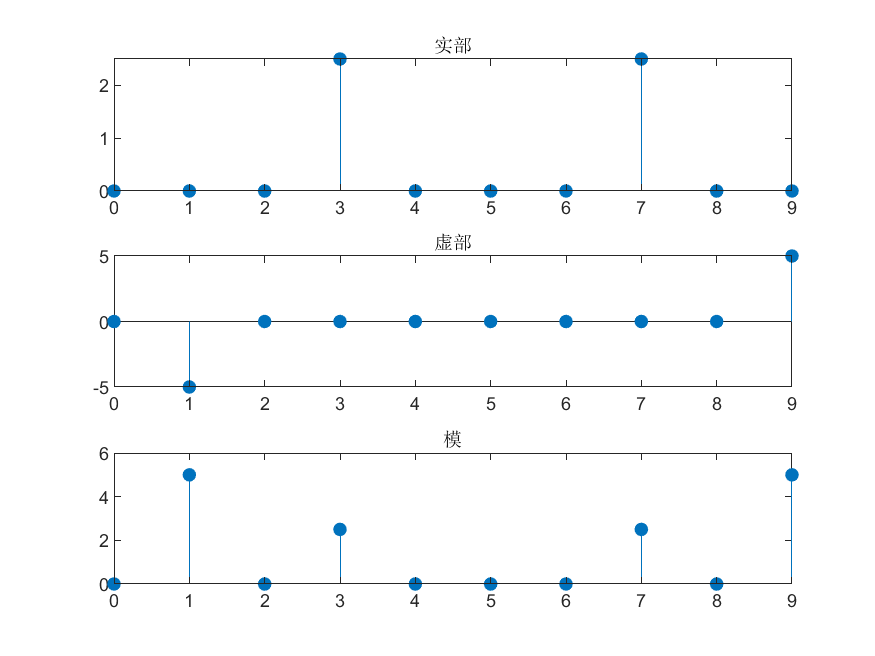
\includegraphics[width=\textwidth]{figure/频谱_复合函数序列_phi=90.png}
                    \end{minipage}
                    \caption{phi=90}
                \end{figure}

                \newpage

                \begin{figure}[htbp]
                    \centering
                    \begin{minipage}[t]{0.48\textwidth}
                    \centering
                    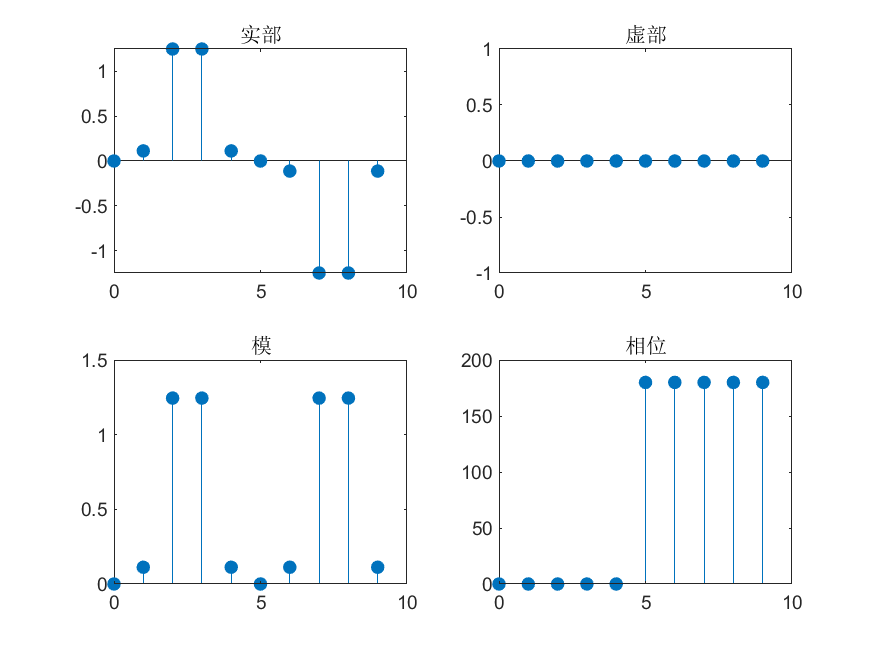
\includegraphics[width=\textwidth]{figure/复合函数序列_phi=180.png}
                    \end{minipage}
                    \begin{minipage}[t]{0.48\textwidth}
                    \centering
                    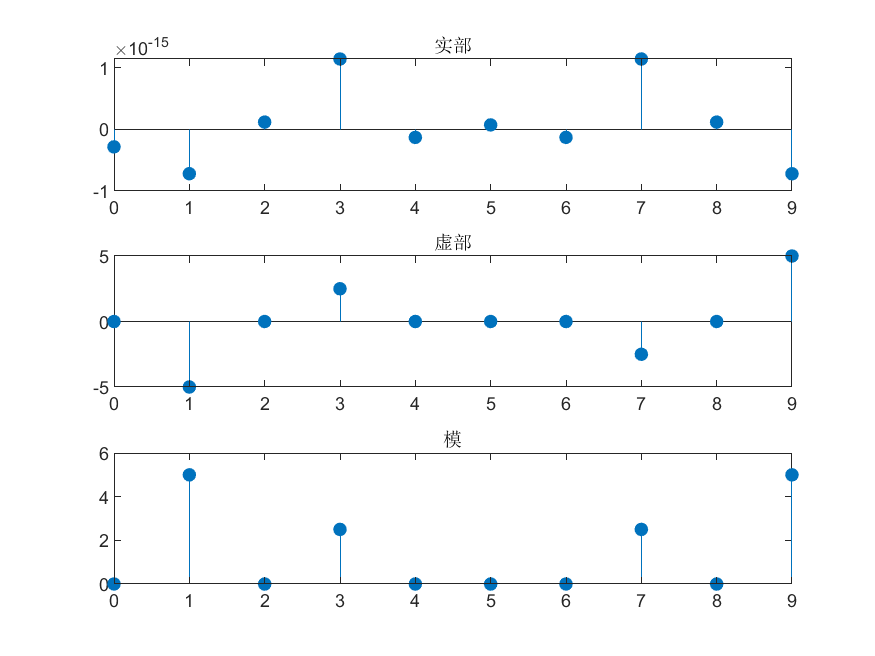
\includegraphics[width=\textwidth]{figure/频谱_复合函数序列_phi=180.png}
                    \end{minipage}
                    \caption{phi=180}
                \end{figure}

                【\textbf{分析}】
                该序列是一个由频率为1Hz和频率为3Hz的两个序列复合而来的实序列,虚部为0.当phi为0和180时,该序列为奇序列,所以频谱实部趋近于0,虚部奇对称。当phi为90时,该序列不具备对称性,所以频谱也不具备对称性。因为复合的序列的频率,所以频域谱线出现在1Hz与3Hz处。

        \subsection{DFT物理意义}
            DFT是序列傅里叶变换在$0-2\pi$上的等距采样。
            \begin{enumerate}
                \item X(0):信号直流分量的频谱值
                \item X(1):信号在基频处的幅度和相位
                \item X(N-1):信号在N-1次谐波处的幅度和相位
            \end{enumerate}

        \subsection{DFT的性质}
            \subsubsection{线性}
            如果$x_1(n)$和$x_2(n)$的DFT为$X_1(k)$与$X_2(k)$,则$ax_1(n)+bx_2(n)$的DFT为$aX_1(k)+bX_2(k)$
            \subsubsection{反转定理}
            如果$x(n)$的DFT结果为$X(k)$,则$x((-n))_N$的DFT为$X((-k))_N$
            \subsubsection{序列的循环位移}
            如果$x(n)$的DFT结果为$X(k)$,则$x((n+m))_N$的DFT为$W_N^{-km}X(k)$
            \subsubsection{对称性}
            见书P_91页
            \subsubsection{卷积性质}
            两个序列圆卷积的DFT等于他们分别DFT的结果相乘
            \subsubsection{帕斯瓦尔定理}
            $$\sum_{n=0}^{N-1}|x(n)|^2 = \frac{1}{N}\sum_{k=0}^{N-1}|X(k)|^2$$

        
            
            



    
\end{document}